
\documentclass{ctexart}
\usepackage[a4paper,hmargin={0.75cm},vmargin={0.75cm}]{geometry}
\usepackage{fancyhdr}
\pagestyle{empty}
\fancyhf{}
\usepackage{tikz}
\usetikzlibrary{shapes,snakes}
\begin{document}
%书法用纸效果:田字格(20*25)

% \noindent

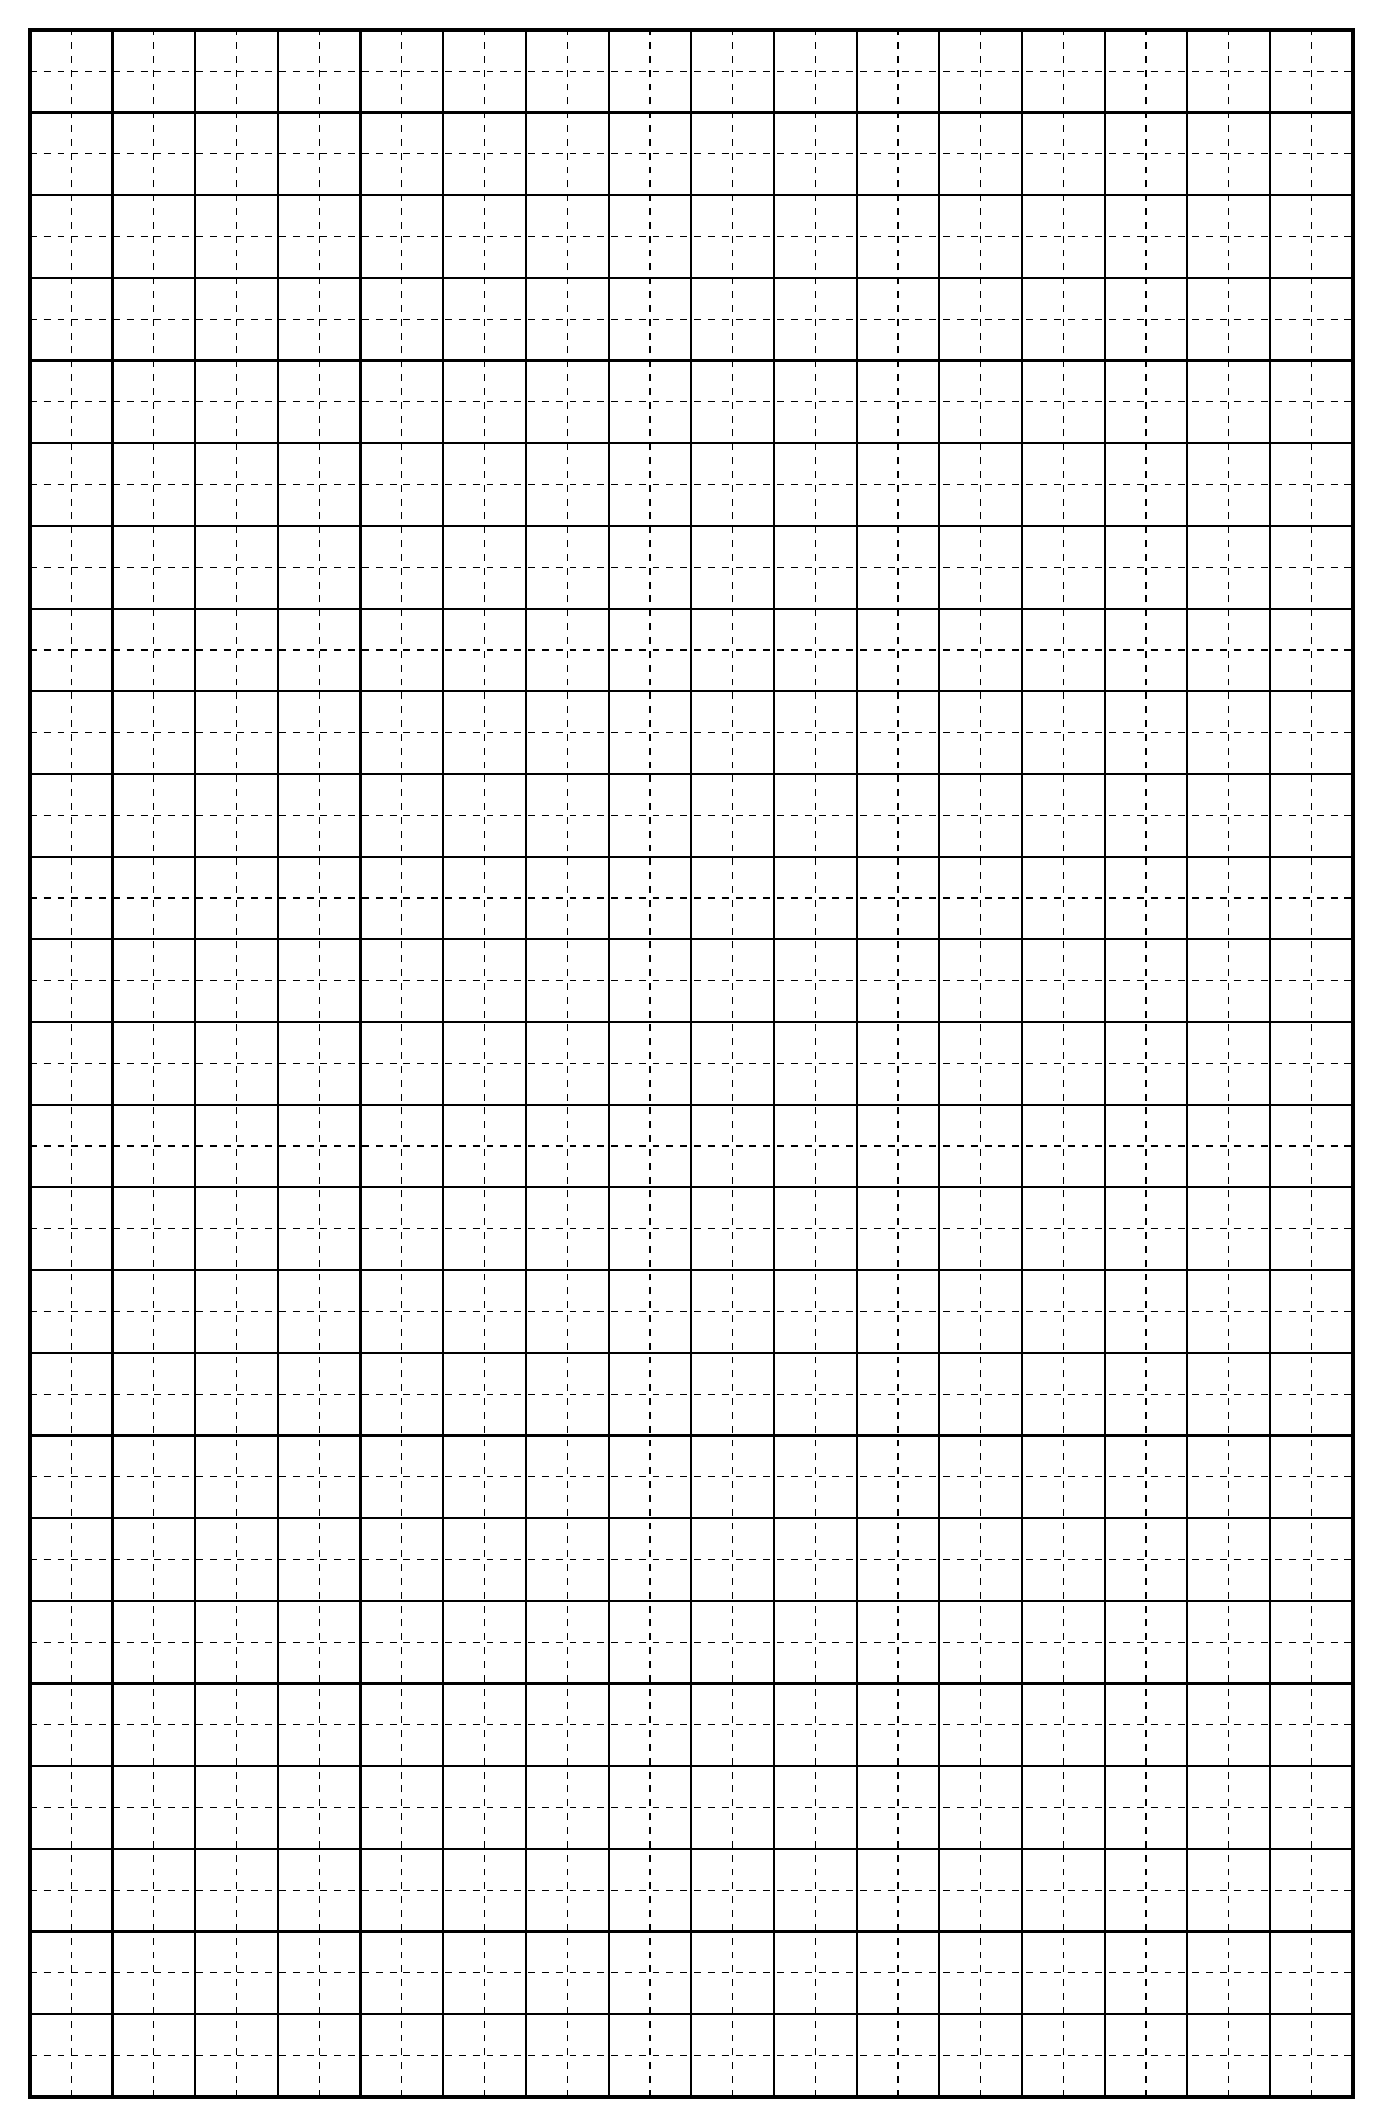
\begin{tikzpicture}[scale=1.05]
\draw[dash pattern=on 2.5pt off 2.5pt](0,0)grid[step=0.5cm](16,25);
\draw[thick](0,0)grid(16,25);
\draw[ultra thick](0,0)rectangle(16,25);
\end{tikzpicture}
\end{document}


\documentclass{ctexart}
\usepackage[b4paper,hmargin={1.5cm},vmargin={2.3cm},landscape]{geometry}
\usepackage{fancyhdr}
\pagestyle{empty}
\fancyhf{}
\usepackage{tikz}
\usetikzlibrary{shapes,snakes}
\begin{document}
%书法用纸效果:田字格, b4paper

\begin{tikzpicture}[scale=1.3]
\draw[dash pattern=on 2.5pt off 2.5pt](0,0)grid[step=0.5](10,14);
\draw[thick](0,0)grid(10,14);
\draw[ultra thick](0,0)rectangle(10,14);
\draw (5,15)node{\bf\scalebox{2}[2.5]{硬笔书法比赛用纸}};
\end{tikzpicture}
\rule{4cm}{0pt}
\begin{tikzpicture}[scale=1.3]
\draw[dash pattern=on 2.5pt off 2.5pt](0,0)grid[step=0.5](10,14);
\draw[thick](0,0)grid(10,14);
\draw[ultra thick](0,0)rectangle(10,14);
\draw (5,15)node{\bf\scalebox{2}[2.5]{硬笔书法比赛用纸}};
\end{tikzpicture}
\end{document}


\documentclass{ctexart}
\usepackage[b4paper,hmargin={2cm},vmargin={2.3cm},landscape]{geometry}
\usepackage{fancyhdr}
\pagestyle{empty}
\fancyhf{}
\usepackage{tikz}
\usetikzlibrary{shapes,snakes}
\begin{document}
%书法用纸效果:米字格, b4paper

\begin{tikzpicture}[scale=1.3]
\draw (5,15)node{\bf\scalebox{2}[2.5]{硬笔书法比赛用纸}};
\clip (0,0)rectangle(10,14);
\foreach \t in {-9,-8,...,13}\draw[very thin,dash pattern=on 2.5pt off 2.5pt] plot[domain=0:10](\x,\x+\t);
\foreach \t in {0,1,...,23}\draw[very thin,dash pattern=on 2.5pt off 2.5pt] plot[domain=0:10](\x,-\x+\t);
\draw[dash pattern=on 2.5pt off 2.5pt](0,0)grid[step=0.5](10,14);
\draw[thick](0,0)grid(10,14);
\draw[ultra thick](0,0)rectangle(10,14);
\end{tikzpicture}
\rule{3cm}{0pt}
\begin{tikzpicture}[scale=1.3]
\draw (5,15)node{\bf\scalebox{2}[2.5]{硬笔书法比赛用纸}};
\clip (0,0)rectangle(10,14);
\foreach \t in {-9,-8,...,13}\draw[very thin,dash pattern=on 2.5pt off 2.5pt] plot[domain=0:10](\x,\x+\t);
\foreach \t in {0,1,...,23}\draw[very thin,dash pattern=on 2.5pt off 2.5pt] plot[domain=0:10](\x,-\x+\t);
\draw[dash pattern=on 2.5pt off 2.5pt](0,0)grid[step=0.5](10,14);
\draw[thick](0,0)grid(10,14);
\draw[ultra thick](0,0)rectangle(10,14);
\end{tikzpicture}
\end{document}
